\documentclass[11pt]{article}      
\usepackage[a4paper,                
top=1in,                         
bottom=1in,                       
left=1in,                         
right=1in]{geometry} 

\setlength\parindent{0pt}
                                    
\usepackage[english]{babel}
\usepackage{amsfonts} 
\usepackage{amsmath}
\usepackage{amsthm}
\usepackage{amssymb}
\usepackage{mathtools} 
\usepackage{graphicx} 
\usepackage{xcolor}
\usepackage{bbm}
\usepackage{float}
\usepackage{verbatim}
\usepackage{tikz}
\usepackage{subcaption}

\usepackage[colorlinks=true, linkcolor=blue]{hyperref}
\usepackage{hyperref}

\usepackage{tikz}
\usetikzlibrary{shapes.geometric, positioning}
\usetikzlibrary{arrows.meta, positioning, calc}

\thinmuskip=4mu
\medmuskip=6mu
\thickmuskip=8mu

\begin{document}
\begin{figure}[t!]
\centering
\includegraphics[width=60mm]{Latex/logoEPFL.png}
\end{figure}

\begin{center}
{\Large \textbf{Numerical Flow Simulation  - Project 1}}\\
\vspace{2mm}
{\large Yanpeng Zhang, Stefano Bernasconi, Pietro Fumagalli, Francesco Derme}\\
{\large 394469, 4141363, 414991, 394806}
\end{center}

\vspace{2.5pt}
\paragraph{Setup.}
Consider a fluid flowing through a plane channel between horizontal walls located in $y = 0$ and $y = H$ as shown in Figure \ref{channel_domain}. The temperature field $T(x, y)$ is the solution of the steady heat equation, $\nabla\cdot(\rho\,u\,T)=\nabla\cdot(\Gamma\,\nabla T)$. Here, the density $\rho$, the velocity field $u$=$[u_x , u_y]^T$ and the thermal properties are known ($\Gamma = k/c_p$ is the ratio of thermal conductivity $k$ to specific heat capacity $c_p$). Assume that $T$ is a passive scalar, i.e. the fluid properties and the velocity field are independent of temperature. The two-dimensional numerical domain is a simple rectangle such that $0 \leq x\leq L$ and $0 \leq y \leq H$. Also, consider a structured mesh with $n_x$ cells in the $x$ direction and $n_y$ cells in the $y$ direction, then $\Delta x = L/(n_x-1)$, $\Delta y = H/(n_y-1)$. Here, the denominator is $n_x - 1$ instead of $n_x$ because the boundary control volumes, as will be explained later, are cut in half so that their nodes sit exactly on the inlet, outlet or the walls. Indices $i, j$ range from 1 to $n_y, n_x$ respectively. By convention, the origin $(x,y)=(0,0)$ corresponds to the upper-left corner of the domain and thus to the center of the upper-left control-volume which is indexed by $(i,j)=(1,1)$, while $(i,j)=(n_y,n_x)$ are the indexes of the center of the bottom-right CV.
\begin{figure}[h!]
    \centering
    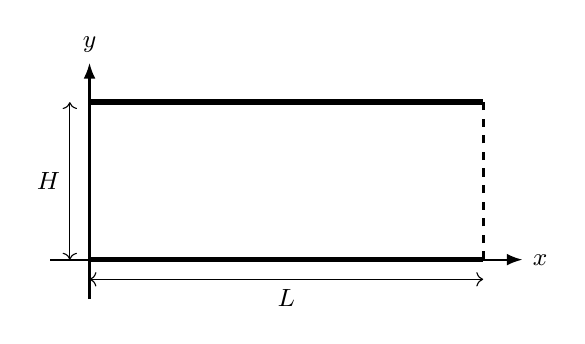
\begin{tikzpicture}[
        scale=0.5,
        font=\small
    ]
        \coordinate (origin) at (0,0);
        \coordinate (L_end) at (10,0);
        \coordinate (H_end) at (0,4);  
        \coordinate (LH_end) at (10,4);

        \draw[line width=2pt, fill=gray!10] (origin) -- (L_end);
        \draw[line width=2pt, fill=gray!10] (H_end) -- (LH_end);
        
        %\draw[dashed, line width=1pt] (origin) -- (H_end);
        \draw[dashed, line width=1pt] (L_end) -- (LH_end);

        \draw[->, thick, -{Latex[length=2mm]}] (-1,0) -- (11, 0) node[right] {$x$};
        \draw[->, thick, -{Latex[length=2mm]}] (0,-1) -- (0, 5) node[above] {$y$};
        %\node[below left=1mm and 1mm] at (origin) {$(0,0)$};

        \draw[<->] (0, -0.5) -- (10, -0.5);
        \node[below] at (5, -0.5) {$L$};
        \draw[<->] (-0.5, 0) -- (-0.5, 4);
        \node[left] at (-0.5, 2) {$H$};

    \end{tikzpicture}    
    \caption{Schematic of the 2D plane channel flow domain.}
    \label{channel_domain}
\end{figure}


\bigskip

\textbf{1. Fully developed laminar velocity.}
Consider the Navier-Stokes equations for the steady, incompressible case. Mathematically, to be \textit{fully developed} means $\partial_x u_x=0 \land \partial_x u_y=0$. Then, the spanwise momentum equation gives $\partial_y p=0$ and the continuity equation is $\partial_y u_y = \partial_x u_x = 0 \implies u_y$ is constant, so $u_y \equiv 0$ since $u_y(0) = u_y(H) = 0$ by the no-slip condition. The streamwise momentum equation instead reduces to
\[
0=-\frac{\mathrm{d}p}{\mathrm{d}x}+\mu\,\frac{\mathrm{d}^2 u_x}{\mathrm{d}y^2},
\]
subject to $u_x(0)=u_x(H)=0$. Integrating twice and applying boundary conditions gives
\[
u_x(y)=-\frac{1}{2\mu}\frac{\mathrm{d}p}{\mathrm{d}x}\,y(H-y),
\]
by symmetry the maximum lies at $y=H/2$
\[
u_{\max}=-\frac{1}{8\mu}\frac{\mathrm{d}p}{\mathrm{d}x}H^2.
\]
The mean velocity can be computed as
\[
u_{\mathrm{mean}}=\frac{1}{H}\int_0^{H}u_x(y)\,\mathrm{d}y=-\frac{1}{12\mu}\frac{\mathrm{d}p}{\mathrm{d}x}H^2,
\]
leading to to $u_{\max}=\tfrac{3}{2}\,u_{\mathrm{mean}}$. Finally,
\begin{align*}
u_x(y) &= u_{\max}\!\left[1 - \Bigl(2\frac{y}{H}-1\Bigr)^2\right] = 4u_{\max}\,\frac{y}{H}\!\left(1 - \frac{y}{H}\right) \\
u_x(y) &= 6u_{\mathrm{mean}}\,\frac{y}{H}\!\left(1 - \frac{y}{H}\right)\\
u_y(y) &= 0
\end{align*}

\bigskip

\textbf{2. Integral form on one CV.}
Consider the steady heat equation $\nabla\cdot(\rho\,u\,T)=\nabla\cdot(\Gamma\,\nabla T)$, integrating over an inner control volume of size $\Delta x\times\Delta y$ centered at $(i,j)$, and applying the divergence theorem gives
\begin{align*}
& \int_{\mathrm{CV}} \nabla\!\cdot(\rho\,u\,T) \,dV = \int_{\mathrm{CV}} \nabla\!\cdot(\Gamma\,\nabla T) \,dV\\
&\int_{\partial \mathrm{CV}} \rho(uT)\cdot n\,\mathrm{d}S=\int_{\partial \mathrm{CV}} \Gamma\,\nabla T\cdot n\,\mathrm{d}S\\
&\int_{ \mathrm{n}} \rho(u_yT)\,\mathrm{d}S - \int_{ \mathrm{s}} \rho(u_yT)\,\mathrm{d}S + \int_{ \mathrm{e}} \rho(u_xT)\,\mathrm{d}S - \int_{ \mathrm{w}} \rho(u_xT) \,\mathrm{d}S=\\
&\int_{ \mathrm{n}} \Gamma\,\partial_y T\,\mathrm{d}S-\int_{ \mathrm{s}} \Gamma\,\partial_y T\,\mathrm{d}S+\int_{\ \mathrm{e}} \Gamma\,\partial_x T\,\mathrm{d}S-\int_{\ \mathrm{w}} \Gamma\,\partial_x T\,\mathrm{d}S&
\end{align*}

Where the east, west, north, and south faces are as shown in Figure \ref{fvm_grid_exact}. Pay attention not to mix the symbols $\mathrm{n}$, which refers to the north face, and $n$, which is the outward unit normal to the surface $\partial \mathrm{CV}$.
\begin{figure}[h!]
    \centering
    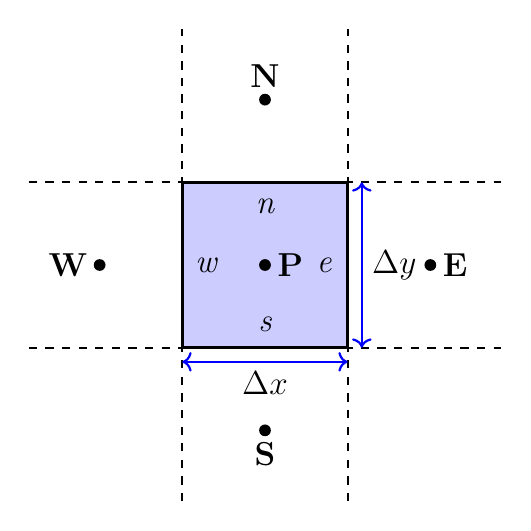
\begin{tikzpicture}[
        scale=0.6,
        font=\large,
        cv_node/.style={
            fill=black, 
            circle, 
            inner sep=1.5pt
        },
        node_label/.style={
            font=\large\bfseries,
            inner sep=2pt
        },
        face_label/.style={
            font=\large\itshape,
            inner sep=1pt
        }
    ]
        \def\nodedist{3.5cm}
        \def\grid_extent{5cm}
        
        \draw[dashed, line width=0.8pt] (-\grid_extent, \nodedist/2) -- (\grid_extent, \nodedist/2);
        \draw[dashed, line width=0.8pt] (-\grid_extent, -\nodedist/2) -- (\grid_extent, -\nodedist/2);
        \draw[dashed, line width=0.8pt] (\nodedist/2, -\grid_extent) -- (\nodedist/2, \grid_extent);
        \draw[dashed, line width=0.8pt] (-\nodedist/2, -\grid_extent) -- (-\nodedist/2, \grid_extent);

        \draw[line width=1.0pt, fill=blue!20] 
            (-\nodedist/2, -\nodedist/2) rectangle (\nodedist/2, \nodedist/2);
        
        \node[cv_node, label={[node_label]right:P}] (P) at (0,0) {};
        \node[cv_node, label={[node_label]above:N}] (N) at (0, \nodedist) {};
        \node[cv_node, label={[node_label]below:S}] (S) at (0, -\nodedist) {};
        \node[cv_node, label={[node_label]right:E}] (E) at (\nodedist, 0) {};
        \node[cv_node, label={[node_label]left:W}] (W) at (-\nodedist, 0) {};
        
        \node[face_label] at (\nodedist/2 - 0.5cm, 0) {e};
        \node[face_label] at (-\nodedist/2 + 0.5cm, 0) {w};
        \node[face_label] at (0, \nodedist/2 - 0.5cm) {n};
        \node[face_label] at (0, -\nodedist/2 + 0.5cm) {s};

        \draw[<->, thick, blue] 
            (\nodedist/2 + 0.3cm, -\nodedist/2) -- (\nodedist/2 + 0.3cm, \nodedist/2) 
            node[midway, right, text=black] {$\Delta y$};
        
        \draw[<->, thick, blue] 
            (-\nodedist/2, -\nodedist/2 - 0.3cm) -- (\nodedist/2, -\nodedist/2 - 0.3cm) 
            node[midway, below, text=black] {$\Delta x$};
            
    \end{tikzpicture}
    
    \caption{The 2D FVM grid notation.}
    \label{fvm_grid_exact}
\end{figure}

\bigskip

\textbf{3. Discretization at faces.}
We approximate the surface integrals from the previous point using the values at the faces' centers
\[
(F_n T_n - F_s T_s) + (F_e T_e - F_w T_w)
=(J^{\text{diff}}_n - J^{\text{diff}}_s) + (J^{\text{diff}}_e - J^{\text{diff}}_w),
\]
where $F_e=(\rho\,u_x)|_e\,\Delta y$ and $J_e^\text{diff}=(\Gamma\,\partial_xT)|_e\,\Delta y$ are the convective and diffusive fluxes through the eastern face and the others are defined similarly. Now we interpolate face values from nodal values. For the diffusive fluxes, we apply central differencing
\begin{alignat*}{2}
&J^{\text{diff}}_e = \Gamma\,\frac{T_E-T_P}{\Delta x}\,\Delta y
= D_e\,(T_E-T_P), \qquad &&D_e=\Gamma\frac{\Delta y}{\Delta x},\\
&J^{\text{diff}}_w = \Gamma\,\frac{T_P-T_W}{\Delta x}\,\Delta y
= D_w\,(T_P-T_W), \qquad &&D_w=\Gamma\frac{\Delta y}{\Delta x},\\
&J^{\text{diff}}_n = \Gamma\,\frac{T_N-T_P}{\Delta y}\,\Delta x
= D_n\,(T_N-T_P), \qquad &&D_n=\Gamma\frac{\Delta x}{\Delta y},\\
&J^{\text{diff}}_s = \Gamma\,\frac{T_P-T_S}{\Delta y}\,\Delta x
= D_s\,(T_P-T_S), \qquad &&D_s=\Gamma\frac{\Delta x}{\Delta y}
\end{alignat*}

And for the convective fluxes, with upwind differencing
\begin{align*}
T_e=
\begin{cases}
T_P,&F_e>0,\\
T_E,&F_e<0
\end{cases}
\qquad
T_w=
\begin{cases}
T_W,&F_w>0,\\
T_P,&F_w<0
\end{cases}
\end{align*}
Since $u_y = 0$, $F_n = F_s = 0$.

\bigskip

\textbf{4. Algebraic equation in an inner CV.}
The discretized flux balance reads
\[
a_P\,T_P=a_E\,T_E+a_W\,T_W+a_N\,T_N+a_S\,T_S+b_P
\]
where
\begin{alignat*}{2}
&a_E = D_e + \max(-F_e,0), \qquad &&a_W = D_w + \max(F_w,0),\\
&a_N = D_n, \qquad &&a_S = D_s,\\
&a_P = a_E+a_W+a_N+a_S+(F_e-F_w), \qquad &&b_{i,j} =0
\end{alignat*}

Once again, $u_y = 0 \implies F_n = F_s = 0$ and, by the continuity equation in the incompressible case, $F_e = F_w$ so $a_P$ has one less term. Physically, each term is a flux times temperature, in fact, using the fundamental measures $[\mathrm{M}]=\text{mass},\;[\mathrm{L}]=\text{length},\;[\mathrm{T}]=\text{time},\;[\mathrm{K}]=\text{temperature}$, we have
\begin{align*}
&[k]=\frac{\mathrm{W}}{\mathrm{m\,K}}=\frac{\mathrm{kg}\,\mathrm{m}}{\mathrm{s}^3\,\mathrm{K}} = \frac{[\mathrm{M}][\mathrm{L}]}{[\mathrm{T}]^3[\mathrm{K}]}\\
&[c_p]=\frac{\mathrm{J}}{\mathrm{kg\,K}}=\frac{\mathrm{m}^2}{\mathrm{s}^2\,\mathrm{K}} = \frac{[\mathrm{L}]^2}{[\mathrm{T}]^2[\mathrm{K}]}\\
&[\Gamma]=\frac{[k]}{[c_p]}=
\frac{\dfrac{[\mathrm{M}][\mathrm{L}]}{[\mathrm{T}]^3[\mathrm{K}]}}
{\dfrac{[\mathrm{L}]^2}{[\mathrm{T}]^2[\mathrm{K}]}}
= \frac{[\mathrm{M}]}{[\mathrm{L}][\mathrm{T}]} \;=\; [M][L]^{-1}[T]^{-1}\\
&[D_e]=[\Gamma]\frac{[\Delta y]}{[\Delta x]}
=[M][L]^{-1}[T]^{-1}\frac{[L]}{[L]}
=[M][L]^{-1}[T]^{-1}\\
&[F_e]=[\rho][u][\Delta y]
=[M][L]^{-3} \cdot [L][T]^{-1}[L]
=[M][L]^{-1}[T]^{-1}
\end{align*}
therefore
\[
[a_E] =[D_e + \max(-F_e,0)] = [M][L]^{-1}[T]^{-1}
\]
By similar computations for the other coefficients, we conclude that
\[
[a_P\,T_P]=[a_E\,T_E]=[a_W\,T_W]=[a_N\,T_N]=[a_S\,T_S]=[M][L]^{-1}[T]^{-1}[K],
\]
The unit of $b$ is not computed since it is everywhere equal to 0.

\bigskip

\textbf{5. CV indexing and boundaries.}
Consider the mesh described in Figure \ref{fvm_grid_exact}, we assign indices to the control volumes in the following manner
\begin{align*}
&i=1,\dots,n_y \quad\text{(spanwise direction, from upper to lower wall)},\\
&j=1,\dots,n_x \quad\text{(streamwise direction, from inlet to outlet)}
\end{align*}

The boundaries are
\[
\begin{cases}
\text{Inlet: } (i,j) = (i,1), & i\in\{1,\dots,n_y\},\\
\text{Outlet: } (i,j) = (i,n_x), & i\in\{1,\dots,n_y\},\\
\text{Lower wall: } (i,j) = (n_y, j), & j\in\{1,\dots,n_x\},\\
\text{Upper wall: } (i,j) = (1, j), & j\in\{1,\dots,n_x\}
\end{cases}
\]

An inner CV indexed by $(i,j)$ has neighbors:
\[
\begin{aligned}
W &\equiv (i,j-1) \quad &\text{(west neighbor)},\\
E &\equiv (i,j+1) \quad &\text{(east neighbor)},\\
S &\equiv (i+1,j) \quad &\text{(south neighbor)},\\
N &\equiv (i-1,j) \quad &\text{(north neighbor)}.
\end{aligned}
\]
With this convention \(W\) and \(E\) are located along the streamwise ($x$) direction, \(S\) and \(N\) are along the spanwise ($y$) direction, and the origin \((x,y)=(0,0)\) corresponds to the center of the top–left CV at the intersection between channel inlet and upper wall. The convention is outlined in Figure \ref{indexing_sketch_split}.
\begin{figure}[h!]
    \centering % Center the figure
    
    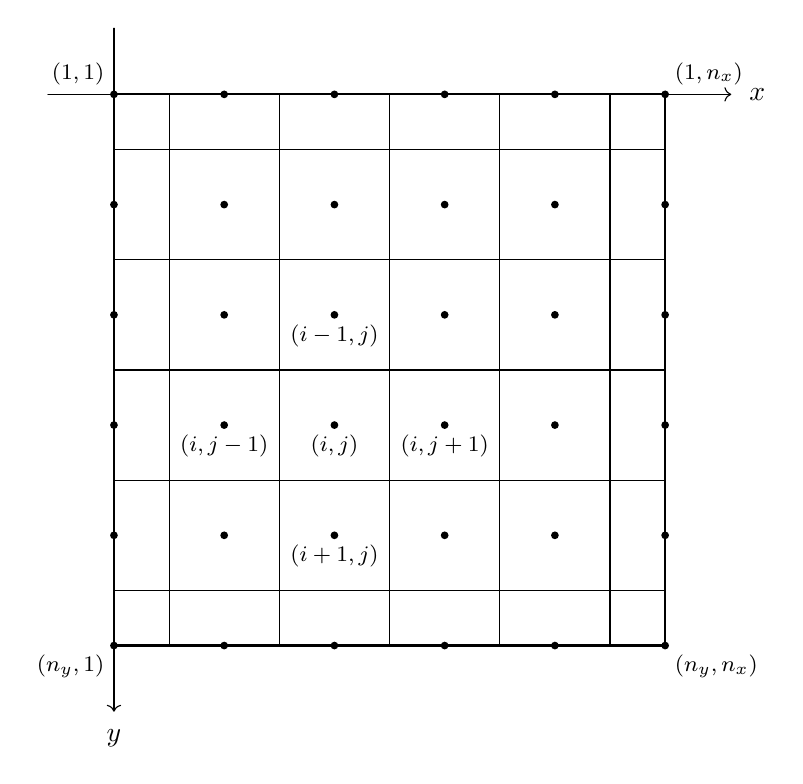
\begin{tikzpicture}[scale=1.4, line cap=round, line join=round]
        % parameters
        \def\nx{6}   % number of centers along x   (i = 1..nx)
        \def\ny{6}   % number of centers along y   (j = 1..ny)
        \def\dx{1} % interior-cell edge in x     (distance between centers)
        \def\dy{1} % interior-cell edge in y

        % domain frame: centers (1,1) at (0,0), (nx,ny) at ((nx-1)dx,(ny-1)dy)
        \pgfmathsetmacro{\xmin}{0}
        \pgfmathsetmacro{\ymin}{0}
        \pgfmathsetmacro{\xmax}{(\nx-1)*\dx}
        \pgfmathsetmacro{\ymax}{(\ny-1)*\dy}

        % external rectangle
        \draw[thick] (\xmin,\ymin) rectangle (\xmax,\ymax);

        % internal faces are mid-planes between adjacent centers
        % vertical faces
        \foreach \k in {1,...,\numexpr\nx-1\relax}{
            \pgfmathsetmacro{\x}{(\k-0.5)*\dx}
            \draw (\x,\ymin) -- (\x,\ymax);
        }
        
        % horizontal faces
        \foreach \l in {1,...,\numexpr\ny-1\relax}{
            \pgfmathsetmacro{\y}{(\l-0.5)*\dy}
            \draw (\xmin,\y) -- (\xmax,\y);
        }

        % centers: first layer lies on the frame, corners included
        \foreach \i in {1,...,\nx}{
            \foreach \j in {1,...,\ny}{
                \pgfmathsetmacro{\xc}{(\i-1)*\dx}
                \pgfmathsetmacro{\yc}{(\j-1)*\dy}
                \fill (\xc,\yc) circle (1-2pt);
            }
        }

        % axes
        \draw[->] (\xmin-0.6,\ymax) -- (\xmax+0.6,\ymax) node[right=3pt] {$x$};
        \draw[->] (0,\ymax+0.6) -- (0,\ymin-0.6) node[below=3pt] {$y$};

        % key labels
        \node[below left]   at (\xmin,\ymin) {\footnotesize $(n_y,1)$};
        \node[below right]  at (\xmax,\ymin) {\footnotesize $(n_y,n_x)$};
        \node[above left]   at (\xmin,\ymax) {\footnotesize $(1,1)$};
        \node[above right]  at (\xmax,\ymax) {\footnotesize $(1,n_x)$};

        % example generic (i,j)
        \pgfmathsetmacro{\xg}{(\nx>3 ? 2*\dx : \dx)}
        \pgfmathsetmacro{\yg}{(\ny>3 ? 2*\dy : \dy)}
        \node[below] at (\xg,\yg) {\footnotesize $(i,j)$};

        \pgfmathsetmacro{\xg}{(\nx>3 ? \dx : \dx)}
        \node[below] at (\xg,\yg) {\footnotesize $(i,j-1)$};

        \pgfmathsetmacro{\xg}{(\nx>3 ? 3*\dx : \dx)}
        \node[below] at (\xg,\yg) {\footnotesize $(i,j+1)$};

        \pgfmathsetmacro{\xg}{(\nx>3 ? 2*\dx : \dx)}
        \pgfmathsetmacro{\yg}{(\ny>3 ? \dy : \dy)}
        \node[below] at (\xg,\yg) {\footnotesize $(i+1,j)$};

        \pgfmathsetmacro{\yg}{(\ny>3 ? 3*\dy : \dy)}
        \node[below] at (\xg,\yg) {\footnotesize $(i-1,j)$};
    \end{tikzpicture}
    
    \caption{Indexing convention.}
    \label{indexing_sketch_split}
\end{figure}

\bigskip

\textbf{6. DOF numbering and mapping.}
Once discretized, the unknown $T$ is a vector of $N = n_x \cdot n_y$ values. We number these $N$ degrees of freedom (DOFs) by flattening $(i,j)$ into a single index $n$ with row-major, top-to-bottom ordering
\[
n = (i-1)\,n_x + j=1,\dots,n_x n_y
\]
For a generic inner CV of DOF index $n$, its neighbors are
\[
E:n+1,\quad W:n-1,\quad N:n-n_x,\quad S:n+n_x
\]
While the boundary DOFs are
\begin{alignat*}{2}
&\text{Inlet: } n = (i-1)n_x + 1, \qquad&& i \in \{1,\dots,n_y\}, \\
&\text{Outlet: } n = (i-1)n_x + n_x, \qquad&& i \in \{1,\dots,n_y\}, \\
&\text{Lower wall: } n = (n_y-1)n_x + j, \qquad&& j \in \{1,\dots,n_x\}, \\
&\text{Upper wall: } n = j, \qquad&&j \in \{1,\dots,n_x\}
\end{alignat*}

\bigskip

\textbf{7. Assembly of the matrix A and Inlet Boundary.}
With our convention, the equation of the the n-th control volume $a_P\,T_P=a_W\,T_W+a_E\,T_E+a_S\,T_S+a_N\,T_N+b_P$ becomes
$$a_{n,n-n_x}\,T_{n-n_x} + a_{n,n-1}\,T_{n-1}+a_{n,n}\,T_{n}+a_{n,n+1}\,T_{n+1}+a_{n,n+n_x}\,T_{n+n_x}=b_n$$
This linear system of equations is described by a matrix $A\in \mathbb{R}^{N\times N}$ and a vector $b\in \mathbb{R}^N$ whose entries, for inner CVs, are
\begin{align*}
&A(n, n) = a_P, \quad A(n, n+1) = -a_E, \quad A(n, n-1) = -a_W, \\
&A(n, n+n_x) = -a_N, \quad A(n, n-n_x) = -a_S, \quad b(n) = 0
\end{align*}
At the inlet boundary (\(1 \leq i \leq n_y\), \(j=1\)), \(T = T_{\text{in}}\), thus
\[
A(n, :) = 0, \quad A(n, n) = 1, \quad b(n) = T_{\text{in}}, \quad \text{where } n = (i-1)n_x + 1
\]

\bigskip

\textbf{8. Outlet Boundary.}
For outlet CVs (\(1 \leq i \leq n_y\), \(j = n_x\)), the Neumann condition \(\partial T/\partial x = 0\) leads to $a_E = 0$. Numerically
\begin{align*}
&A(n, n) = a_P, \quad A(n, n+1) = 0, \quad A(n, n-1) = -a_W, \quad A(n, n+n_x) = -a_N, \\
&A(n, n-n_x) = -a_S, \quad b(n) = 0, \quad \text{where } n = (i-1)n_x + n_x
\end{align*}

\bigskip

\textbf{9. Wall Boundaries.}
For lower wall (\(i=n_y\), \(1 \leq j \leq n_x\)) and upper wall (\(i = 1\), \(1 \leq j \leq n_x\)) CVs, \(T = T_{\text{wall}}\), so
\[
A(n, :) = 0, \quad A(n, n) = 1, \quad b(n) = T_{\text{wall}}, \quad \text{where } n = j \lor n=(n_y-1)n_x + j
\]
Note that corner CVs (e.g., \((i=1,j=1)\)) are assigned to walls to avoid boundary condition conflicts.

\bigskip

\textbf{10. Physical Parameter Calculation.}
Consider the following values for the fluid's physical properties: $\rho = 1\ \text{kg/m}^3$, $c_p = 10\ \text{J/(K $\cdot$ kg)}$, $k = 0.12\ \text{W/(m $\cdot$ K)}$, $\nu = 10^{-2}\ \text{m}^2/\text{s}$. Assume also that $L = 10\ \text{m}$, $H = 1\ \text{m}$, then $\mathrm{Pe} = \rho \cdot u_\text{mean} \cdot (2H) / \Gamma = 16.5$.

\begin{align*}
    &\Gamma = \frac{k}{c_p} = \frac{0.12}{10} = 0.012\ \frac{\text{kg}}{m \cdot \text{s}}, \\
    &u_{\text{mean}} = \frac{Pe \cdot \Gamma}{2H \cdot \rho} = \frac{16.5 \cdot 0.012}{2 \cdot 1 \cdot 1} = 0.099\ \text{m/s}, \\
    &\mathrm{Re} = \frac{2H u_{\text{mean}}}{\nu} = \frac{2 \cdot 1 \cdot 0.099}{10^{-2}} = 19.8
\end{align*}

Since Re is much lower than the threshold value of 2300, so the flow is expected to be laminar.

\bigskip

\textbf{11. Coarse Mesh Solution and Visualization.}
Assume $T_\text{inlet} = 50^\circ C$ and $T_\text{wall} = 100^\circ C$. On a coarse mesh with \(n_x = 50\), \(n_y = 5\), the temperature field results physically reasonable, as shown in Figure \ref{temperature_field}.

\begin{figure}[H]
    \centering
    \includegraphics[width=1\textwidth]{Latex/MATLABfigures/11.png} 
    \caption{Channel temperature field (\(n_x=50\), \(n_y=5\)).}
    \label{temperature_field}
\end{figure}

\textbf{12. Boundary conditions verification.}
As demonstrated by the plots in Figure \ref{boundary_condition}, the solution respects all boundary conditions. Indeed we can see that: for the inlet the solution assumes the value $T_\text{wall} = 100^\circ C$ at the edges and the value $T_\text{inlet} = 50^\circ C$ for the internal nodes; at the outlet the functions $T(x,0.75)$ and $T(x,0.5)$ becomes flat when they reach $L=10\,m$, this means that their derivative with respect to x, at the end of the channel, is zero, as stated by the Neumann conditions; for the two horizontal walls is clear that the value remain constant to $T_\text{wall} = 100^\circ C$ both at $y=0$ and $y=H$.

\begin{figure}[H]
    \centering
    \includegraphics[width=0.9\textwidth]{Latex/MATLABfigures/12.png} 
    \caption{Top left plot shows how our solution assumes the inlet boundary condition; bottom left and bottom right respectively show how our solution correctly assumes the boundary conditions for the lower and upper wall; top right plot shows streamwise temperature evolution of our solution evaluated at two different heights (y=0.75, y=0.5), indeed we observe a Neumann condition at x=L.}
    \label{boundary_condition}
\end{figure}

\textbf{13. Temperature plots.} 
The 2D plot of the solution $T(x,y)$ can be seen in Figure \ref{temperature_field}. The outlet temperature is shown in Figure \ref{outlet_temperature}, while in Figure \ref{cent_mean_temp} the centerline temperature and the weighted mean temperature are plotted together with the entry length ($x_e = 2.449$). Note that the weighted mean temperature, defined as follows, is computed numerically, summing up all the contributions over the spanwise direction, in order to approximate the two integrals.

\begin{align}
    T_{mean}(x) = \dfrac{\int_{0}^{H}u_x(y)T(x,y)dy}{\int_{0}^{H}u_x(y)dy}
    \label{T_mean_formula}
\end{align}

\begin{figure}[H]
    \centering
    \includegraphics[width=0.6\textwidth]{Latex/MATLABfigures/13_1.png} 
    \caption{Temperature field at the outlet.}
    \label{outlet_temperature}
\end{figure}

\begin{figure}[H]
    \centering
    \includegraphics[width=0.6\textwidth]{Latex/MATLABfigures/13_2.png} 
    \caption{Centerline and velocity-weighted mean temperature.}
    \label{cent_mean_temp}
\end{figure}

\textbf{14. Iterative methods.} 
In order to solve the system $AT=b$, instead of the Matlab backslash, we implement the Successive Over Relaxation method: starting from a suitable initial guess $T^0$, that respect the boundary conditions (for example a $T^0$ equal to $50^\circ C$ on the inlet and $100^\circ C$ on the two walls), the method monitors the values of relative iteration error $||T^k - T^{k-1}||_2\,/\,||T^{k-1}||_2 $ (Figure \ref{relative_error}), and the normalized residuals $||AT^k - b||_2\,/\,||diag(A)\,T^k||_2 $ (Figure \ref{residuals}), and stop when both are smaller than the tolerance $10^{-5}$. The SOR method is an algorithm that includes a relaxation parameter, $w$, to control its convergence. The choice of this parameter is critical: setting $w=1$ simplifies the algorithm to the standard Gauss-Seidel method. In contrast, setting w in the range $1<w<2$ (in this case, $w=1.5$) applies over-relaxation, a technique designed to accelerate convergence. The simulation using the Gauss-Seidel method took 35 iterations to meet the stopping criteria, while the over-relaxation method converged significantly faster, requiring only 23 iterations.

\begin{figure}[H]
    \centering
    \includegraphics[width=0.7\textwidth]{Latex/MATLABfigures/14_1.png} 
    \caption{Temperature field at the outlet.}
    \label{relative_error}
\end{figure}

\begin{figure}[H]
    \centering
    \includegraphics[width=0.7\textwidth]{Latex/MATLABfigures/14_2.png} 
    \caption{Centerline and velocity-weighted mean temperature.}
    \label{residuals}
\end{figure}

\textbf{15. Nusselt Number computation}
Consider the Nusselt Number defined as 
\begin{align}
    \mathrm{Nu} = \frac{\partial T / \partial n}{\Delta T / (2H)}
    \label{nusselt_formula}
\end{align}
where $\Delta T = T_{wall}\,-T_{mean}$ is the difference between the wall temperature and the velocity-averaged mean temperature $T_{mean}$ defined earlier. For laminar flows in plane channels, as shown by \cite{nusselt}, $\mathrm{Nu}(x)$ decreases in the entrance region, but far enough downstream of the inlet it approaches a constant value independent of the Péclet number. To remark that we're working in the case of uniform wall temperature, the Nusselt number is indicated as $\mathrm{Nu_T}(x)$. Numerically, we compute $\mathrm{Nu_T}(x)$ by approximating the velocity-averaged mean temperature (as in question 13) and the normal derivative of the temperature at the wall using a finite difference, the resulting $\mathrm{Nu_T}(x)$ along the lower wall can be observed in Figure \ref{nusselt}. It tends to a limit of 6.68, which we found to be reasonably close to the expected value of 7.54. 

However, contrary to theoretical expectations, the trend also presents a sudden spike in Nusselt value near the outlet. This feature is a numerical artifact, not a physical phenomenon, and is caused by a conflict between the physics of the flow and the Neumann boundary condition. Indeed, a Neumann null outlet condition means that the temperature profile is no longer changing in the direction of the flow. Apparently, this is pacific since it's also what we expect from the definition of \textit{fully developed} flow. In reality, there is still heat transfer occurring at the outlet, so such condition on the gradient is too restrictive, leading to a model incapable of capturing the essence of our phenomenon. 

Numerically, what happens is that the solver has to forcibly bend the temperature profile in the last few cells of the mesh to satisfy the Neumann condition. This distortion then pollutes the entire temperature field upstream of the outlet, rendering the calculated wall gradient smaller than what is expected form experiments, and leading to the artificial spike in the value of $\mathrm{Nu}$ we observe.

\begin{figure}[H]
    \centering
    \includegraphics[width=0.7\textwidth]{Latex/MATLABfigures/15.png} 
    \caption{Nusselt Number along the lower wall.}
    \label{nusselt}
\end{figure}

\textbf{16. Mesh refinement study.} 
To ensure that the numerical solution is independent of the grid resolution, a mesh convergence study was performed. The simulation was run on four progressively refined meshes, as shown in Table \ref{mesh_refinement}. To evaluate the convergence between these cases, several key quantities of interest were computed and compared. These include the outlet temperature profile $T_o(y)$, the centerline temperature $T_c(x)$ and the mean temperature $T_{mean}(x)$ defined by \ref{T_mean_formula}, the entry length $x_e$ and the local Nusselt number $Nu(x)$, defined by \ref{nusselt_formula}, along the heated wall. The results can be seen in the plots below.

\begin{table}[H]
    \centering
        \begin{tabular}{|c|c|c|} 
        \hline
        $\mathbf{n_x}$ & $\mathbf{n_y}$ & \textbf{Entry Length} \\ 
        \hline
        50 & 5 & 2.449 \\ 
        \hline
        100 & 11 & 2.3232 \\ 
        \hline
        200 & 21 & 2.2111 \\ 
        \hline
        400 & 41 & 2.1805 \\
        \hline
        \end{tabular}
    \caption{The Mesh refinement and the corresponding entry length values}
    \label{mesh_refinement}
\end{table}

\begin{figure}[H]
    \centering
    \includegraphics[width=0.6\textwidth]{Latex/MATLABfigures/16_1.png} 
    \caption{}
    \label{}
\end{figure}

\begin{figure}[H]
    \centering
    \includegraphics[width=0.6\textwidth]{Latex/MATLABfigures/16_2.png} 
    \caption{}
    \label{}
\end{figure}

\begin{figure}[H]
    \centering
    \includegraphics[width=0.6\textwidth]{Latex/MATLABfigures/16_3.png} 
    \caption{}
    \label{}
\end{figure}

\begin{figure}[H]
    \centering
    \includegraphics[width=0.6\textwidth]{Latex/MATLABfigures/16_4.png} 
    \caption{}
    \label{}
\end{figure}

\bibliographystyle{plain}
\bibliography{literature}

\end{document}
